\section{PaTAS For Neural Networks}\label{sec:patas}

When neural network parameters such as \( \theta_1 \) and \( \theta_2 \) are learned (e.g., by backpropagation), their trustworthiness depends on the data used for training. If the dataset contains mislabeled or biased samples, parameter trust will be compromised. Yet this is only part of the problem. As discussed in Section~\ref{sec:backsl}, Subjective Logic represents trust as a subjective binomial opinion with the three components trust (belief), distrust (disbelief), and uncertainty. This decomposition allows us to distinguish between different causes of unreliability: distrust may arise from systematic issues such as mislabeled or poisoned data, while uncertainty reflects variability or noise in the assessment. A central challenge, therefore, is how to exploit this advantage of subjective logic in order to make this distinction in practice.

\vspace{-0.5em}
\subsection{PaTAS General Description}

To address the previous challenges, we introduce the \emph{Parallel Trust Assessment System (PaTAS)}, a framework designed to systematically propagate trust assessments through a neural network. PaTAS operates in parallel with the standard neural architecture and maintains a corresponding structure that mirrors the network’s topology. It computes trust in the output from two sources:
\begin{enumerate}
    \item the trust in the input features at inference time, and
    \item the trust in the parameters, derived from the training dataset trustworthiness calculated using a trust assessment function. 
    This includes both the trust in the input features of the training samples and the trust in the labels.
\end{enumerate}
To extend the trust-propagation principles introduced for the perceptron in the previous section, PaTAS organizes its Trust Nodes into a structure that mirrors the full neural network. Each neuron is associated with a corresponding Trust Node, and these nodes are connected according to the network’s topology. This generalization forms what we refer to as a Trust Nodes Network (TNN).
\begin{definition}[Trust Nodes Network]
The \emph{Trust Nodes Network} is a structured composition of Trust Nodes, where each Trust Node corresponds to a neuron in the underlying neural network. This network mirrors the architecture of the neural model and is responsible for propagating trust values across layers. The Trust Nodes Network computes trust assessments at each stage of inference by applying trust-specific reasoning operations aligned with the neural computation flow.
\end{definition}

The PaTAS is designed to continuously evaluate the trustworthiness and preservation of properties, such as accuracy, during the inference of a neural network. For example, an input \(x\) might be accurate, unbiased, and trustworthy (i.e., high trust score value \(T_x\)), while the corresponding output \(y\prime\) may still be unreliable due to biased or poorly calibrated parameters \(\theta\) (i.e., low trust score value \(T_{y\prime}\)). Rather than altering the neural network itself, PaTAS operates alongside it to evaluate the trustworthiness of computations (Appendix~\ref{app:flow}). Embedding trust operations inside the network would modify its internal computations, risk harming accuracy, and substantially increase the computational cost. For this reason, PaTAS performs trust assessment in parallel, ensuring that trust reasoning does not interfere with the model’s predictions or complicate its operation.




\vspace{-0.5em}
\subsection{PaTAS Design}
\begin{figure}
    \centering
    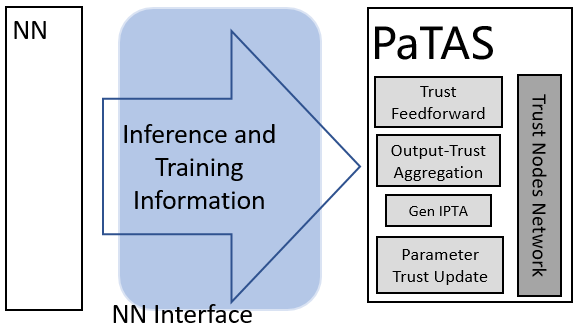
\includegraphics[width=0.62\linewidth]{good_figs/ptas/highPaTAS.png}
    \caption{High-Level Overview of PaTAS Integration with a Neural Network}
    \label{fig:highptas}
\end{figure}

% \subsection{PaTAS Components}\label{sec:ptasarch}



As illustrated in~\cref{fig:highptas}, PaTAS is composed of four main modules: Trust Feedforward, Output-Trust Aggregation, GenIPTA, 
and Parameter-Trust Update. 
Among these, the Parameter-Trust Update requires a more detailed treatment, 
since its design parallels the role of backpropagation in neural network training 
and involves elaborate reasoning operations. 
We therefore dedicate a separate subsection to it.
\subsubsection{Trust Feedforward}

The Trust Feedforward function propagates trust through the Trust Node Network in alignment with the model's inference flow, mirroring its layer-wise computation but operating on trust values: at each layer, input and parameter trust are combined through the Trust Function's discounting and fusion. It produces a trust opinion for each output neuron and stores the intermediate trust scores later used by the Parameter-Trust Update.

\subsubsection{Output-Trust Aggregation}

Output-Trust Aggregation combines the per-neuron output opinions into a single trust score via an SL fusion operator. Alternatively, one may read off the trust of the decided class directly: in digit classification, if the model predicts class `1', the decision trust is the opinion of that output Trust Node.

\subsubsection{Inference-Path Trust Assessment Generation(GenIPTA)}

GenIPTA dynamically constructs, for a single inference, a function called Inference-Path Trust Assessment (IPTA) that reflects the trustworthiness of the exact computational path taken. The activation trace recorded during that inference instantiates a temporary subnetwork containing only the Trust Nodes of the activated neurons, mirroring the precise inference path. 

Since all neurons are typically activated to some degree while only a subset is strongly relevant, GenIPTA can also operate on truncated activation sets retaining the most relevant neurons, or weight the assessment by the actual activation values so that stronger activations contribute more heavily.

The detailed functional flow of PaTAS across feedforward, backpropagation, and inference is illustrated in Appendix~\ref{app:flow}.

\vspace{-0.5em}
\subsection{Parameter-Trust Update}\label{sec:ptasfunc}
The Parameter-Trust Update adapts the trust of model parameters during training so that it reflects both the model's observed behavior and the reliability of the training data. To ground the design, recall the standard gradient-descent update for a parameter $\theta$:
\begin{equation}
\label{eq:gd1}
\theta \leftarrow \theta - l_r  \frac{\partial \mathcal{L}}{\partial \theta},
\end{equation}
where $l_r$ is the learning rate, $\mathcal{L}$ is the loss function, and $\frac{\partial \mathcal{L}}{\partial \theta}$ is the gradient. These gradients are computed recursively using the chain rule:
\begin{equation}
\label{eq:gd2}
\frac{\partial \mathcal{L}}{\partial \theta^{(l)}_{i,j}}
= \delta^{(l)}_i x^{(l-1)}_j,
\end{equation}
where $\theta^{(l)}_{i,j}$ denotes the weight connecting neuron $j$ in layer $(l-1)$ to neuron $i$ in layer $l$, $\delta^{(l)}_i$ is the error term of neuron $i$, and $x^{(l-1)}_j$ is the activation from the previous layer.

In particular, \cref{eq:gd2} shows that gradients factor into an error term and an input activation, revealing that parameter updates depend jointly on gradient signals, input activations, and learning dynamics. PaTAS mirrors this structure by incorporating gradient information, input feature trust, and label trust as evidence in the Parameter-Trust Update.

The notation used throughout this subsection is summarized in \cref{tab:params-appendix} in Appendix~\ref{app:symbols}, and the complete update procedure is given in \cref{alg:trustupdate}.

\begin{algorithm}
\caption{Parameter-Trust Update. Revises the trust of each Trust Node parameter by combining gradient evidence, label trust, and neuron input trust under mini-batch training. Helper functions are given in Appendix~\ref{app:algorithm}.}
\begin{algorithmic}[1]
    \Function{ParameterTrustUpdate}{$g, T_y, \epsilon$}
        \State $T_{y_\text{batch}}  \longleftarrow  \bigwedge_{y \in y_\text{batch}} T_y$ \Comment{aggregate label trust}
        \For{each layer $l$}
            \For{each neuron $n_i^{(l)}$}
                \State $g^{(l)}_i  \longleftarrow  \{\, g^{(l)}_{i,j} \;|\; j \in \mathcal{N}(i)\,\}$
                \State $T_{n_i \mid y_\text{batch}}  \longleftarrow $ \Call{NodeTrust}{$g^{(l)}_i, T_{y_\text{batch}}, \epsilon$}
                \State $T_{n_i \parallel Y_\text{batch}}  \longleftarrow $ \Call{DeduceTrust}{$T_{n_i \mid y_\text{batch}}, T_{n_i \mid \overline{y_\text{batch}}}, T_{y_\text{batch}}$}
                \For{each incoming edge $j$ to $n_i^{(l)}$}
                    \State $T_{\theta_{i,j}^{(l)}}  \longleftarrow $ \Call{Revise}{$T_{\theta_{i,j}^{(l)}}, T_{n_i \parallel Y_\text{batch}}$}
                    \State $T_{\theta_{i,j}^{(l)}} \longleftarrow $ \Call{Update}{$T_{\theta_{i,j}^{(l)}}, T_{x^{(l-1)}_j}, T_{y_\text{batch}}$}
                \EndFor
            \EndFor
        \EndFor
    \EndFunction
\end{algorithmic}
\label{alg:trustupdate}
\end{algorithm}
The procedure in \cref{alg:trustupdate} runs once per mini-batch and iterates over all layers and neurons. It first aggregates label trust, \(T_{y_\text{batch}} = \bigwedge_{y \in y_\text{batch}} T_y\), which conditions the trust in every parameter. For each neuron \(n_i^{(l)}\) it then derives \( T_{n_{i}^{(l)} \mid y_\text{batch}} \) from gradient evidence, counting each incoming weight gradient with \( |g^{(l)}_{i,j}| < \epsilon\)\footnote{The threshold $\epsilon$ is not a tuned hyperparameter but a sensitivity parameter used only in \textsc{NodeTrust} to separate weak from strong gradients; we select it relative to the typical gradient scale during training. It does not affect model predictions or training dynamics, only the sensitivity of the trust update.} as positive evidence \(r\) and the remainder as negative evidence \(s\), and mapping \((r,s)\) to a binomial opinion via \cref{eq:q1}. Since no evidence is available for the complementary case, \( T_{n_{i}^{(l)} \mid \overline{y_\text{batch}}} \) is vacuous, and the deduction operator \( \circledcirc \) combines the two conditionals with \( T_{y_\text{batch}} \) to give \( T_{n_{i}^{(l)} \parallel Y_\text{batch}} \).

For each incoming edge \(j\), the parameter trust is then revised with the deduced neuron trust, \(T_{\theta_{i,j}^{(l)}} \leftarrow T_{\theta_{i,j}^{(l)}} \circleddash T_{n_{i}^{(l)} \parallel Y_\text{batch}}\), and adjusted for the auxiliary factors that also drive the gradient update in \cref{eq:gd1,eq:gd2}, namely the learning rate, the input feature, and the batch labels:
\begin{equation}
    T_{\theta_{i,j}^{(l)}} \longleftarrow T_{\theta_{i,j}^{(l)}} \odot (T_{x_j^{(l)}} \oslash T_{y_\text{batch}}),
\end{equation}
where $\odot$ is binomial multiplication and $\oslash$ is the conservative combination \((b,d,u)\) with \(b = \min(b_1,b_2)\), \(d = \max(d_1,d_2)\), \(u = 1-(b+d)\). This reflects that both unreliable features and mislabeled data can strongly bias parameter updates: trust cannot exceed the weakest evidence and distrust must reflect the strongest warning.

This process refines the trust in each parameter by incorporating both gradient-based behavioral evidence and auxiliary trust factors, allowing the PaTAS to align parameter trust with the training dynamics of the neural network. 

The mapping from gradient magnitude to evidence deserves explicit justification, since a large gradient does not, in isolation, imply an untrustworthy parameter. Two points make the interpretation well founded in PaTAS. First, evidence is \emph{relative}: gradients are not thresholded against an absolute constant but against the prevailing gradient scale through $\epsilon$, so the update reacts to a parameter that keeps receiving atypically large corrections \emph{after} the model has otherwise settled, not to the large gradients that are normal early in training. Second, evidence is \emph{conditional on label trust}: the same large gradient leads to a negative update of the trust assigned to the parameters only insofar as it is driven by data the model trusts. Under trusted labels, a parameter that the network must repeatedly and strongly correct is one whose learned value the trusted data does not support, which is precisely the signal PaTAS accumulates as reduced trust. Under distrusted or uncertain labels, the deduction through $T_{y_\text{batch}}$ discounts that same signal proportionally; the asymptotic cases are summarized in Appendix~\ref{app:asymptotic}. Gradient magnitude is nonetheless a proxy and can be confounded by learning-rate schedules, mini-batch noise, or saddle-point regions; a more direct evidence model for parameter reliability, together with an ablation over $\epsilon$ and gradient statistics, is left to future work.

\paragraph*{Computational Overhead}
PaTAS runs in parallel with the primary network and mirrors its computational flow over subjective opinions, so the total runtime is \(T_{\text{with PaTAS}} = T_{\text{comm}} + \max(T_{\text{PaTAS}}, T_{\text{NN}})\), where \(T_{\text{comm}}\) is the communication overhead between the two. Each PaTAS operation manipulates a four-component opinion rather than a scalar, giving \(T_{\text{PaTAS}} \approx 3\,T_{\text{NN}}\) and hence \(T_{\text{with PaTAS}} \approx T_{\text{comm}} + 3\,T_{\text{NN}}\). Because training requires no value from PaTAS, the neural network can proceed while trust assessment completes.

\vspace{-0.5em}
\subsection{Theoretical Properties of PaTAS}\label{sec:ptastheory}
To ensure that PaTAS provides reliable and interpretable trust assessments, we first establish several fundamental theoretical properties describing its stability and consistency.
\subsubsection{Convergence of PaTAS}
% \todo[inline]{Discuss convergence of PaTAS in case of convergence of input}
\label{sec:ptas_convergence}

The convergence of the PaTAS is governed by the stability of its inputs and the structure of its recursive Parameter-Trust Update process. During training, PaTAS updates the internal trust opinions associated with network parameters using trust opinions on the inputs, labels, hyperparameters, and gradient information. This update mechanism is outlined in \cref{alg:trustupdate}. As proved in Theorem~\ref{thm:convergence}, the PaTAS converges under specific situation. This convergence relies on some specific characteristic of the operators used to feedforward and revise the trust in the parameters \(\theta\). 

% Before delving into the specifics of PaTAS convergence, we first present a key theorem that will serve as a foundational tool in establishing the convergence properties of PaTAS.


\begin{theorem}[Convergence of PaTAS Creation]\label{thm:convergence}
\footnote{All proofs of the theorems in this section, as well as additional theoretical results, are provided in the \suppp.}

Let a neural network be trained until convergence, and let its associated PaTAS operate with:

\begin{itemize}
    \item a stable input trust assessment $T_x$,
    \item a stable label trust assessment $T_y$,
    \item a stable hyperparameter $\epsilon$.
    % \item and converging back propagation gradients $g$.
\end{itemize}

Let $T_\theta^{(n)}$ denote the trust opinion at iteration $n$ for parameter $\theta$. If the revision of the trust in the weights is performed as specified in \cref{alg:trustupdate}, then the PaTAS parameter will converge.
\end{theorem}
\subsubsection{Symmetry and Invariance Properties of PaTAS}\label{sec:ptassyminv}

\begin{theorem}[Consistency Properties of PaTAS]\label{thm:infvac}
Let \(\omega^\emptyset=(0,0,1,a)\) be a vacuous binomial opinion and let \(\bar{x}=(d,b,u,a)\) denote the symmetric counterpart of \(x=(b,d,u,a)\). Then, for any parameter trust configuration \(T_\theta\):
\begin{enumerate}
    \item \emph{Vacuity is preserved.} Discounting a vacuous opinion is vacuous, \(\omega^A_B \otimes \omega^\emptyset = \omega^\emptyset\), and hence \(\mathrm{IPTA}(\omega^\emptyset) = \omega^\emptyset\).
    \item \emph{Inference is symmetric.} The outputs \(y = T_\theta(x)\) and \(\bar y = T_\theta(\bar x)\) satisfy \(u_y = u_{\bar y}\), \(b_y = d_{\bar y}\), and \(d_y = b_{\bar y}\). In particular a fully trusted input \((1,0,0)\) yields \(d_y = 0\), and a fully distrusted input \((0,1,0)\) yields \(b_{\bar y} = 0\).
\end{enumerate}
\end{theorem}

These properties act as consistency guarantees rather than as the paper's headline result: they establish that the trust computation is well behaved, propagating vacuity and preserving symmetry under the chosen operators, and thereby justify reasoning about only the trusted-input case in the evaluation. Stronger, security-specific guarantees, such as provable bounds on trust degradation under a bounded poisoning adversary, are not claimed here and are identified as future work.
